\documentclass[a4paper,12pt]{report}

%Русский язык
\usepackage[T2A]{fontenc}
\usepackage[utf8]{inputenc}
\usepackage[english,russian]{babel}
\usepackage{cmap}

%Работа с кодом
\usepackage{listings}
\usepackage{color}

\definecolor{green}{rgb}{0,0.6,0}
\definecolor{gray}{rgb}{0.5,0.5,0.5}
\definecolor{red}{rgb}{0.6,0,0}

\lstset{
        language=Python, 
        basicstyle=\small\ttfamily, 
        numberstyle=\tiny,           
        columns=flexible,
        stepnumber=1,                   
        numbersep=5pt,        
        showspaces=false,
        showstringspaces=false,
        showtabs=false,
        tabsize=2,                
        captionpos=b,              
        breaklines=true,           
        breakatwhitespace=false,
        keywordstyle=\color{green},
        commentstyle=\color{gray},
        stringstyle=\color{red},      
}

%Математика
\usepackage{amsmath,amsfonts,amssymb,amsthm,mathtools} 

%Изображения
\usepackage{float}
\usepackage{graphicx}
\graphicspath{ {./img/} }

%Поля страницы
\usepackage{geometry} 
\geometry{left=2.3cm} 
\geometry{right=1.8cm} 
\geometry{top=2cm} 
\geometry{bottom=2.5cm} 

%Отступы
\usepackage{indentfirst}
\setlength{\parskip}{0cm}

\begin{document} 

\begin{titlepage}
\newpage
	\begin{center}
		\large Санкт-Петербургский политехнический университет Петра Великого\\
		Институт компьютерных наук и технологий\\
		Высшая школа интеллектуальных систем и суперкомпьютерных технологий\\
	\end{center}
\vspace{7cm}

\begin{center}
		\large \textbf{Отчёт по лабораторной работе №5} \\
		\textbf{Дисциплина:} Телекоммуникационные технологии\\
		\textbf{Тема:} Автокорреляция
\end{center}
\vspace{4cm}
	
\begin{flushright}
		\large Работу выполнил:\\ Ляшенко В.В.\\
		Группа: 3530901/80201\\
		Преподаватель:\\ Богач Н.В.
\end{flushright}

\vspace{\fill}
\begin{center}
	\large Санкт-Петербург\\ 2021
	\end{center}
\end{titlepage}

\tableofcontents
\listoffigures
\lstlistoflistings

\chapter{Упражнение 5.1}
    Блокнот Jupyter \texttt{chap05.ipynb} содержит приложение, в котором можно вычислить автокорреляции для различных \texttt{lag}. Воспользуемся им и оценим высоту тона вокального чирпа для нескольких времен начала сегмента. 
    
    Для начала скачаем запись с чирпом и выделим небольшой сегмент.
\begin{lstlisting}[caption=Получение сегмента]
       wave = read_wave('28042__bcjordan__voicedownbew.wav')
       wave.normalize()
       segment = wave.segment(start=0.1, duration=0.01)
\end{lstlisting} 

    Теперь используем автокорреляцию (Рис.1.1).
\begin{lstlisting}[caption=Использование автокорреляцию]
       lags, corrs = autocorr(segment)
       plt.plot(lags, corrs)
       decorate(xlabel='Lag (index)', ylabel='Correlation')
\end{lstlisting}
\begin{figure}[H]
        \centering
        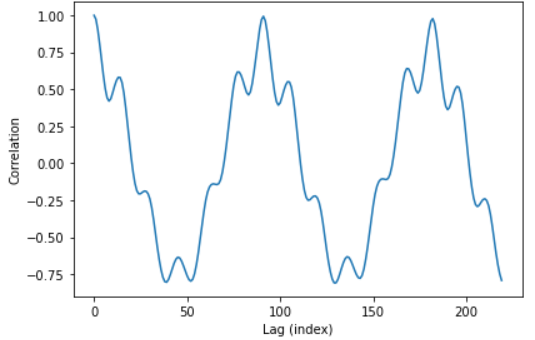
\includegraphics[width=0.8\textwidth]{fig1-1.PNG}
        \caption{Автокорреляция первого сегмента}
        \label{fig:fig1-1}
\end{figure}   
   
    Первый пик находится близко к lag = 100. Уточним значение, используя \texttt{argmax}.
\begin{lstlisting}[caption=Уточнение значения lag]
       low=70
       high=150
       lag = np.array(corrs[low:high]).argmax() + low
       lag
\end{lstlisting}
    
    Полученное значение lag = 91.
    
    Затем вычислим частоту для найденного \texttt{lag}.
\begin{lstlisting}[caption=Нахождение частоты]
       period = lag / segment.framerate
       frequency = 1 / period
       frequency
\end{lstlisting} 
    
     Полученная частота: 485 Гц. 
     
     Возьмем теперь другой сегмент того же сигнала и выполним те же действия (Рис.1.2).
\begin{lstlisting}[caption=Получение сегмента]
       segment2 = wave.segment(start=0.6, duration=0.01)
\end{lstlisting} 
\begin{figure}[H]
        \centering
        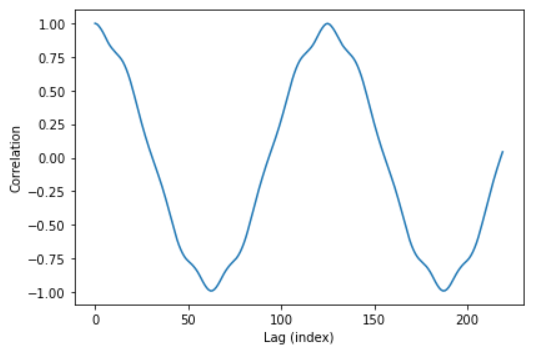
\includegraphics[width=0.8\textwidth]{fig1-2.PNG}
        \caption{Автокорреляция второго сегмента}
        \label{fig:fig1-2}
\end{figure} 

    Полученое значение lag = 125. Полученная частота: 353 Гц. 
    
    Таким образом, при увеличении времени начала сегмента частота уменьшается.

\chapter{Упражнение 5.2}
\section{Функция estimate\_fundamental}
    Пример кода в \texttt{chap05.ipynb} показывает, как использовать автокорреляцию для оценки основной частоты переодического сигнала. Инкапсулируем этот код в функцию, названную \texttt{estimate\_fundamental}.
\begin{lstlisting}[caption=Функция estimate\_fundamental]
       def estimate_fundamental(segment, low=70, high=150):
       lags, corrs = autocorr(segment)
       lag = np.array(corrs[low:high]).argmax() + low
       period = lag / segment.framerate
       frequency = 1 / period
       return frequency
\end{lstlisting}

    Используем ее для отслеживания высоты тона записанного звука. 
\begin{lstlisting}[caption=Применение функции]
       wave = read_wave('28042__bcjordan__voicedownbew.wav')
       wave.normalize()
       segment = wave.segment(start=0.6, duration=0.01)
       freq = estimate_fundamental(segment)
       freq
\end{lstlisting} 

    Полученная частота: 353 Гц.

\section{Спектрограмма}        
    Проверим ее работу функции.
    
    В начале построим спектрограмму записи (Рис.2.1).
\begin{lstlisting}[caption=Построение спектрограммы]
       wave.make_spectrogram(2048).plot(high=4200)
       decorate(xlabel='Time (s)', ylabel='Frequency (Hz)')
\end{lstlisting} 
\begin{figure}[H]
        \centering
        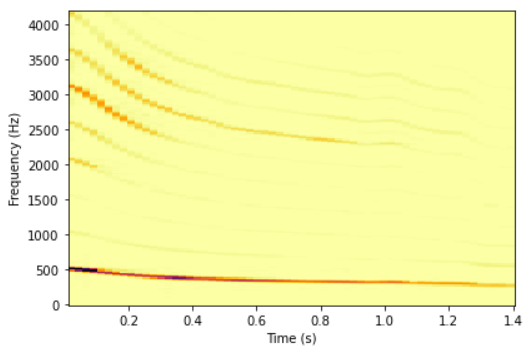
\includegraphics[width=0.8\textwidth]{fig2-1.PNG}
        \caption{Спектрограмма сегмента}
        \label{fig:fig2-1}
\end{figure} 
    
    Теперь будем накладывать оценки высоты на спектрограмму.
\begin{lstlisting}[caption=Наложение оценки высоты на спектрограмму]
       step = 0.05
       starts = np.arange(0.0, 1.4, step)

       ts = []
       freqs = []

       for start in starts:
           ts.append(start + step/2)
           segment = wave.segment(start=start, duration=duration)
           freq = estimate_fundamental(segment)
           freqs.append(freq)

       wave.make_spectrogram(2048).plot(high=900)
       plt.plot(ts, freqs, color='white')
       decorate(xlabel='Time (s)', ylabel='Frequency (Hz)')
\end{lstlisting} 
\begin{figure}[H]
        \centering
        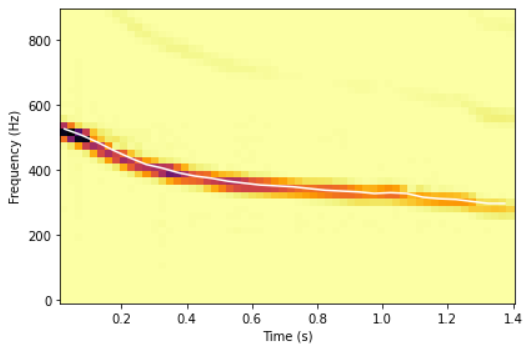
\includegraphics[width=0.8\textwidth]{fig2-2.PNG}
        \caption{Спектрограмма сегмента}
        \label{fig:fig2-2}
\end{figure} 
    
    Как мы можем видеть из рис.2.2, наложение оценки совпадает с кривой на спектрограмме, что говорит нам о правильной работе функции.

\chapter{Упражнение 5.3}
    Используя данные о BitCoin из предыдущей лабораторной (Рис.3.1), вычислим автокорреляцию цен в платежной системе BitCoin.
\begin{lstlisting}[caption=Получение данных о BitCoin]
       import pandas as pd
       from thinkdsp import Wave

       df = pd.read_csv('files/BTC_USD_2020-04-12_2021-04-11-CoinDesk.csv', parse_dates=[0])
       ys = df['Closing Price (USD)']
       ts = df.index
       wave = Wave(ys, ts, framerate=1)
       wave.plot()
       decorate(xlabel='Time (days)')
\end{lstlisting}
\begin{figure}[H]
        \centering
        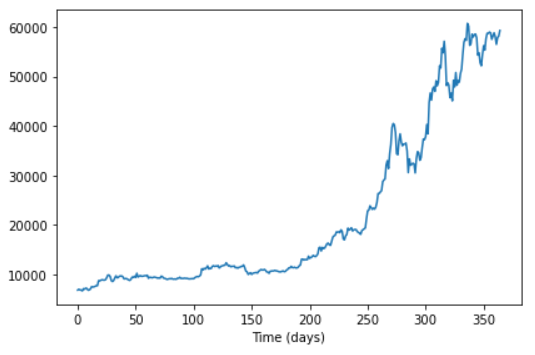
\includegraphics[width=0.8\textwidth]{fig3-1.PNG}
        \caption{Данные о BitCoin}
        \label{fig:fig3-1}
\end{figure} 
    
    Вычислим автокорреляцию.
\begin{lstlisting}[caption=Вычисление автокорреляции]
       lags, corrs = autocorr(wave)
       plt.plot(lags, corrs)
       decorate(xlabel='Lag', ylabel='Correlation')
\end{lstlisting}
\begin{figure}[H]
        \centering
        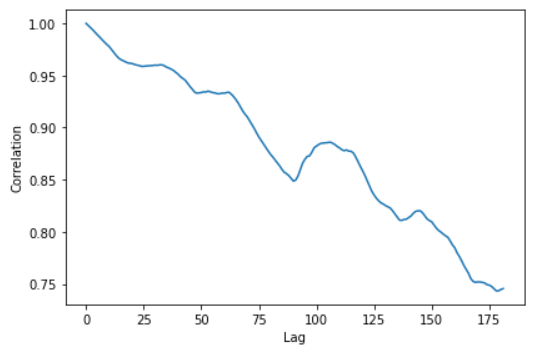
\includegraphics[width=0.8\textwidth]{fig3-2.PNG}
        \caption{Автокорреляция BitCoin}
        \label{fig:fig3-2}
\end{figure} 
     
     Как мы можем видеть на рис.3.2, автокорреляция спадает не очень быстро по мере увеличения задержки, что указывает на то, что перед нами розовый шум.
 
\chapter{Упражнение 5.4}
    Воспользуемся блокнотом \texttt{saxophone.ipynb}, в котором исследуются автокорреляция, восприятие высоты тона и явление под названием «подавленная основная». Запустим примеры из него. Затем выберем другой сегмент записи и вновь поработаем с примерами.
    Пусть новый сегмент будет иметь ту же длину, но начнётся с 5 с.
\begin{lstlisting}[caption=Выделение сегмента]
       start = 5.0
       duration = 0.5
       segment = wave.segment(start=start, duration=duration)
       segment.make_audio()
\end{lstlisting} 

    Построим спектр этого сегмента (Рис.4.1).
\begin{lstlisting}[caption=Построение спектра сегмента]
       spectrum = segment.make_spectrum()
       spectrum.plot(high=3000)
       decorate(xlabel='Frequency (Hz)', ylabel='Amplitude')
\end{lstlisting}
\begin{figure}[H]
        \centering
        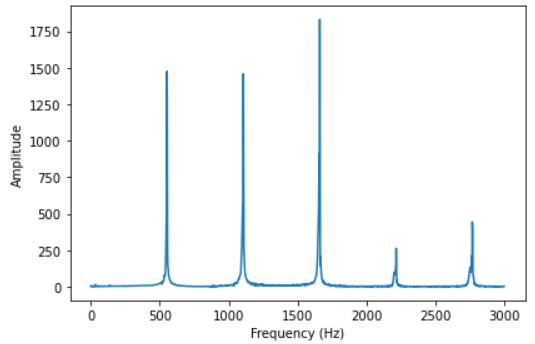
\includegraphics[width=0.8\textwidth]{fig4-1.PNG}
        \caption{Спектр сегмента}
        \label{fig:fig4-1}
\end{figure}

    Затем получим все пики спектра. Пики в спектре находятся на частотах 552, 1106 и 1660 Гц.                    
    
    Высота 552 Гц, которую мы воспринимаем, является основной, но не доминирующей.

    Сравним ее с треугольной волной на частоте 552 Гц.
\begin{lstlisting}[caption=Получение треугольной волны]
       from thinkdsp import TriangleSignal
       TriangleSignal(freq=552).make_wave(duration=0.5).make_audio()
\end{lstlisting}

    У них одинаковая воспринимаемая высота звука.

    Чтобы понять, почему мы воспринимаем основную частоту, даже если она не является доминирующей, используем автокорреляцию.
\begin{lstlisting}[caption=Функция автокорреляции]
       def autocorr(segment):
       corrs = np.correlate(segment.ys, segment.ys, mode='same')
       N = len(corrs)
       lengths = range(N, N//2, -1)

       half = corrs[N//2:].copy()
       half /= lengths
       half /= half[0]
       return half
\end{lstlisting}      
\begin{lstlisting}[caption=Применение функции]
       corrs = autocorr(segment)
       plt.plot(corrs[:200])
       decorate(xlabel='Lag', ylabel='Correlation', ylim=[-1.05, 1.05])
\end{lstlisting}
\begin{figure}[H]
        \centering
        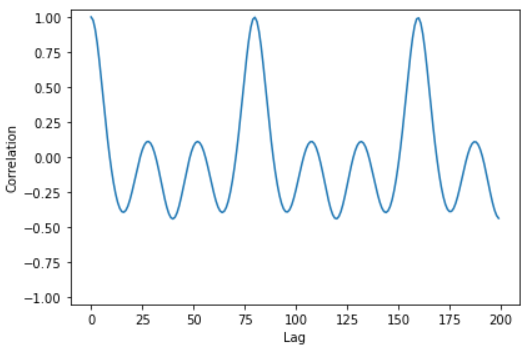
\includegraphics[width=0.8\textwidth]{fig4-2.PNG}
        \caption{Автокорреляция}
        \label{fig:fig4-2}
\end{figure}
    
    Из рис.4.2 мы видим, что первый главный пик находится рядом с lag = 75.
    
    Затем используем функцию \texttt{find\_frequency}, которая находит самую высокую корреляцию в заданном диапазоне задержек и возвращает соответствующую частоту. Находим lag самого высокого пика и его частоту. 
    
    Полученный значения: lag = 80, частота = 551 Гц.
    
    Высота звука, которую мы воспринимаем, соответствует наивысшему пику автокорреляционной функции, а не самому высокому компоненту спектра.
    
    Теперь попробуем удалить основную частоту (Рис.4.3).
\begin{lstlisting}[caption=Удаление освновной частоты]
       spectrum2 = segment.make_spectrum()
       spectrum2.high_pass(600)
       spectrum2.plot(high=3000)
       decorate(xlabel='Frequency (Hz)', ylabel='Amplitude')
\end{lstlisting}
\begin{figure}[H]
        \centering
        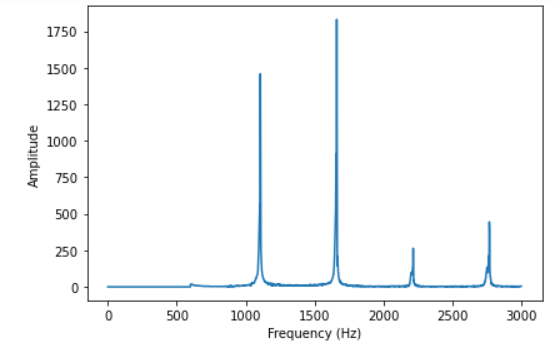
\includegraphics[width=0.8\textwidth]{fig4-3.PNG}
        \caption{Спектр без основной частоты}
        \label{fig:fig4-3}
\end{figure}

    Послушаем полученный сегмент. Воспринимаемая высота звука по-прежнему составляет 551 Гц, хотя на этой частоте нет мощности. Это явление называют «подавленная основная».
    
    Чтобы понять, почему мы слышим частоту, которой нет в сигнале, посмотрим на функцию автокорреляции (Рис.4.4).
\begin{figure}[H]
        \centering
        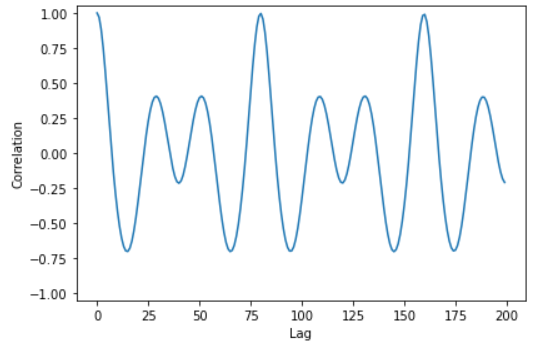
\includegraphics[width=0.8\textwidth]{fig4-4.PNG}
        \caption{Автокорреляция}
        \label{fig:fig4-4}
\end{figure}

    Третий пик, соответствующий 551 Гц, по-прежнему самый высокий.    
    
    Но есть еще два пика, соответствующие 1521 Гц и 558 Гц. Но мы их не воспринимаем, так как высшие компоненты, которые присутствуют в сигнале, представляют собой гармоники 551 Гц, а не гармоники 558 или 1521 Гц.
    
    Наше ухо интерпретирует высокие гармоники как свидетельство того, что «правильная» основная частота составляет 551 Гц.

    Если избавиться от высоких гармоник, эффект исчезнет. Вот спектр с удаленными гармониками выше 1200 Гц (Рис.4.5).
\begin{lstlisting}[caption=Фильтрация гармоник]
       spectrum4 = segment.make_spectrum()
       spectrum4.high_pass(600)
       spectrum4.low_pass(1200)
       spectrum4.plot(high=3000)
       decorate(xlabel='Frequency (Hz)', ylabel='Amplitude')
\end{lstlisting}
\begin{figure}[H]
        \centering
        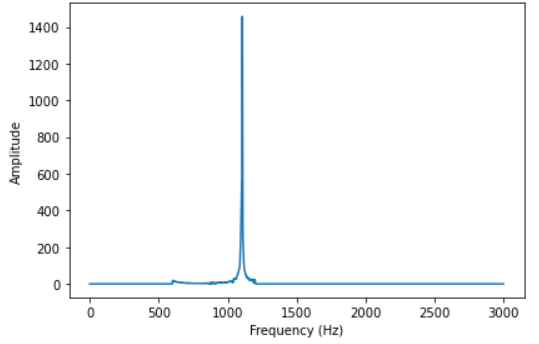
\includegraphics[width=0.8\textwidth]{fig4-5.PNG}
        \caption{Фильтрованный спектр}
        \label{fig:fig4-5}
\end{figure}

\begin{figure}[H]
        \centering
        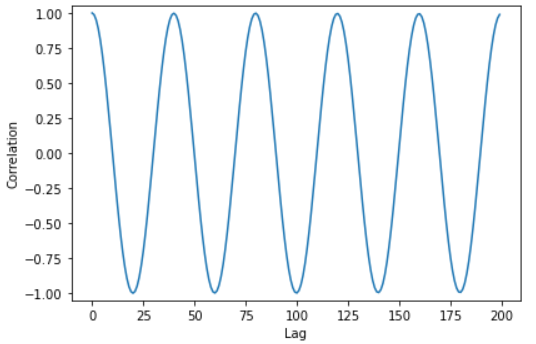
\includegraphics[width=0.8\textwidth]{fig4-6.PNG}
        \caption{Автокорреляция фильтрованного спектра}
        \label{fig:fig4-6}
\end{figure}

    Теперь воспринимаемая высота звука 1106 Гц.Если мы посмотрим на функцию автокорреляции (Рис.4.6), то самый высокий пик будет на lag = 40, что соответствует 1102 Гц.
    
    Таким образом, эти эксперименты показывают, что восприятие высоты звука не полностью основано на спектральном анализе, но также определяется автокорреляцией.
    
\chapter{Выводы}
    В результате выполнения данный работы мы познакомились с понятием автокорреляции и научились использовать ее для оценки высоты тона.
    
    Также мы исследовали понятие «подавленная основная». 
\end{document}